\section{Bargaining over complementary holdings}
\label{sec:bargain}
\subsection{A complete response account}
The corpus contains 526 negotiation threads and 920 responses, comprising 113 acceptances, 394 counters and 413 rejections. Acceptance is legal in 918 cases. Sol and Opus counter most often; Gemini and Grok reject most often. Nevertheless each accepts between 26 and thirty offers. Agreement counts alone conceal the different ways the systems resist or revise proposed terms.

Table~\ref{tab:full} gives every form and completion category at both opening and later stages. Opening proposer-only swaps receive 95/116 rejections, compared with 37/72 for swaps completing neither party, a 30.5-percentage-point gap. Both-party swaps receive 34/48 rejections. Pure cash bids give a different observed comparison, 42/70 versus 67/103, or minus 5.0 points. Their resampling band includes positive and negative differences. The cash estimate is not evidence of a zero population effect.

\begin{table}[t]\centering\small
\begin{tabular}{@{}llrrr@{}}\toprule
Form & Completes & All N (A/C/R) & Opening N (A/C/R) & Later N (A/C/R)\\\midrule
Swap & Proposer only & 155 (8/44/103) & 116 (1/20/95) & 39 (7/24/8) \\
Swap & Recipient only & 47 (12/32/3) & 6 (1/3/2) & 41 (11/29/1) \\
Swap & Both & 81 (10/35/36) & 48 (3/11/34) & 33 (7/24/2) \\
Swap & Neither & 106 (28/34/44) & 72 (17/18/37) & 34 (11/16/7) \\
Cash bid & Proposer only & 131 (11/65/55) & 70 (2/26/42) & 61 (9/39/13) \\
Cash bid & Recipient only & 0 (0/0/0) & 0 (0/0/0) & 0 (0/0/0) \\
Cash bid & Both & 0 (0/0/0) & 0 (0/0/0) & 0 (0/0/0) \\
Cash bid & Neither & 176 (21/75/80) & 103 (4/32/67) & 73 (17/43/13) \\
Other & Proposer only & 3 (0/2/1) & 1 (0/0/1) & 2 (0/2/0) \\
Other & Recipient only & 93 (12/46/35) & 45 (1/15/29) & 48 (11/31/6) \\
Other & Both & 0 (0/0/0) & 0 (0/0/0) & 0 (0/0/0) \\
Other & Neither & 126 (11/60/55) & 63 (3/12/48) & 63 (8/48/7) \\
\bottomrule

\end{tabular}
\caption{All 918 acceptance-legal offers. A, C and R mean accept, counter and reject. Completion is newly acquired after the proposed transfer. The other category includes cash asks to recipients, non-completing unilateral transfers and jail-card bundles. The two acceptance-unavailable responses are outside this common population.}\label{tab:full}
\end{table}

Proposer composition materially changes the magnitude. Grok authors 36/72 neither-completing opening swaps and fifteen of their seventeen acceptances. Excluding all Grok-authored offers leaves 90/108 versus 24/36 rejections, a 16.7-point gap. Deleting only threads initiated by Grok content/call conflicts instead gives 93/112 versus 26/43, a 22.6-point gap. Thirteen of the original seventeen comparator acceptances disappear in that exclusion. These versions answer different descriptive questions. Neither reconstructs the game other players would have encountered without those proposals.

\begin{table}[t]\centering\small
\begin{tabular}{@{}llrr@{}}\toprule
Proposer & Opening form & Proposer-only N (A/C/R) & Neither N (A/C/R)\\\midrule
Sol & Swap & 50 (0/6/44) & 11 (0/2/9) \\
Sol & Cash bid & 13 (0/5/8) & 8 (0/3/5) \\
Gemini & Swap & 8 (0/4/4) & 2 (1/1/0) \\
Gemini & Cash bid & 4 (1/2/1) & 0 (0/0/0) \\
Opus & Swap & 50 (1/7/42) & 23 (1/7/15) \\
Opus & Cash bid & 40 (1/12/27) & 70 (1/18/51) \\
Grok & Swap & 8 (0/3/5) & 36 (15/8/13) \\
Grok & Cash bid & 13 (0/7/6) & 25 (3/11/11) \\
\bottomrule

\end{tabular}
\caption{Proposer strata for the two focal completion categories. All are observed opening offers. Sparse cells and different author proportions limit pooled interpretation; complete recipient strata appear in Appendix~\ref{app:offers}.}\label{tab:proposers}
\end{table}

All four within-proposer swap point differences are positive, but Sol's is only 6.2 points and Gemini has two comparator offers. Standardizing the within-proposer gaps to proposer-only weights gives 16.0 points; neither-cell weights give 21.5; pooled weights give 18.1. A standardized number needs its reference distribution. It also remains a comparison among different properties, compensation, positions and negotiations, rather than an adjustment that identifies concern about rival opportunity.

Across the five seed blocks, swap gaps range from 19.4 to 40.5 points; cash-bid gaps range from minus 22.2 to plus 7.9. Dropping one block leaves swap gaps of 28.7--33.3 and cash gaps of minus 8.3 to minus 2.3. Exact block resampling yields central bands of [24.2, 35.5] for swaps, [-18.0, 3.2] for cash bids and [-3.8, 31.9] for swaps without Grok authors. These relatively narrow or broad bands reflect the observed block profiles and changing offer denominators. With five inspected blocks they are reweighting diagnostics, not confirmation or calibrated predictive intervals.

\begin{figure}[t]\centering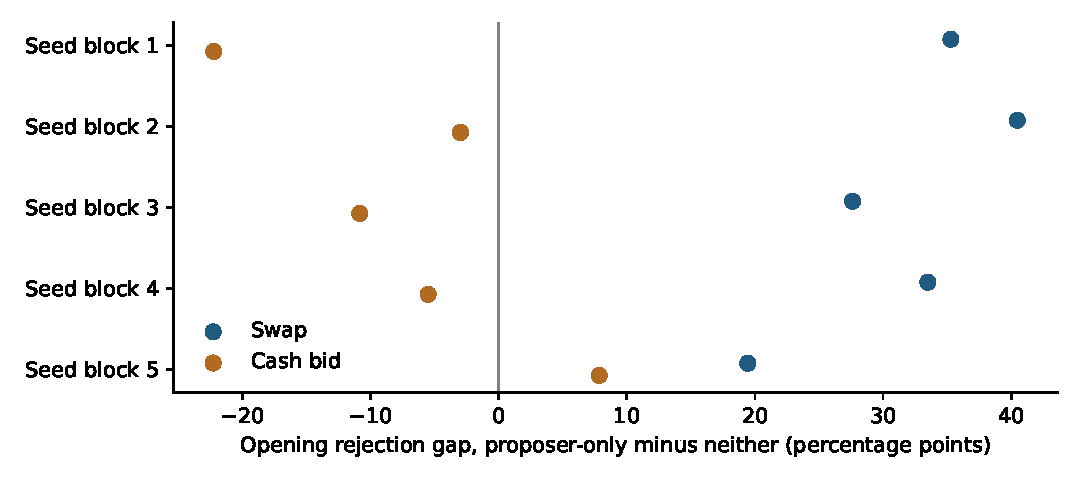
\includegraphics[width=\linewidth]{block_sensitivity.pdf}
\caption{Each seed block's opening rejection gap, using all offers in the two focal cells. The four rotations stay together. Points show observed blocks rather than uncertainty for independent offers; Table~\ref{tab:blocks} prints their denominators.}\label{fig:blocks}
\end{figure}

Recipients may reject unattractive incoming deeds, preserve useful blockers, demand cash, or avoid enabling construction. The records do not hold those consequences fixed. Printed purchase prices normalize units but do not measure the value of a deed with rental, mortgage, complementary and blocking uses. The form split therefore remains economically compositional. Later offers are further selected by previous resistance: later swap rejections are 8/39 versus 7/34, and later cash-bid rejections 13/61 versus 13/73. A smaller later contrast cannot establish that negotiation causes accommodation.

\subsection{Expressed concern in a separate population}
Two retained LLM-assisted readings agree that 61/74 rejected recipient-completing offers name a trade-linked rival consequence. This comprises 27/38 recipient-only and 34/36 both-party rejections. These categories are disjoint from the proposer-only and neither headline comparison. The codes document expressed concern elsewhere; they do not explain the swap/cash gap. Gemini and Grok contribute 56 agreed cases, and G1/G15 contribute 31. One reader had partial exposure to earlier aggregates and a case; agreement is not human validation or a rate of accurate reasoning.

\TranscriptTitle{refusal}{Rejecting one's own complete group}
At G15 turn 63, Sol has \$730 and Grok \$333. Sol offers two greens for Ventnor and \$100, completing both groups. Grok's private note compares development budgets:
\TranscriptQuote{fx-g15-refusal-note}
Sol removes the cash request, then adds Kentucky and finally \$250. Grok still refuses:
\TranscriptQuote{fx-g15-final-refusal}
The first post-trade cash values are correct. A full first green layer costs \$600, but one legal green house costs \$200, so the note should not be read as an inability to build anything. It explicitly weighs immediate rival construction against its own development. All three offers fail. Eighteen turns later Grok's blockers pass to Gemini through bankruptcy; Sol never completes either group. These continuations preserve the stakes without establishing which trade would have been best.
\TranscriptSource{G15 d168--175, standard responses. The quoted public refusal occurs in Sol's next request. The private note is not delivered to Sol.}

This case supports expressed concern, partially checked assessment and action consistency. It does not demonstrate that changing only the rival's opportunity would change the response. The distinction is useful because a refusal can be deliberate, factually grounded and still strategically costly. No counterfactual payoff is assigned to the unaccepted exchange.
